%!TEX root = ../Main.tex

% ------------------------------------------------------------------
\section{Design Process}
Hong and Lancaster~\cite{hong:microstrip} describe a class of filters that would provide the required response if fabricated in high temperature superconducting (HTS) material. As any pre-select filter would need to be installed along with the low noise amplifiers, and cooled to 20K, using superconducting material would make good use of the existing equipment. However, as we did not have the ability to fabricate a HTS device in-house, we decided to first produce a copper prototype to test the theory.

% ------------------------------------------------------------------
\subsection{Quazi-elliptic resonant filters}
The filter design described in~\cite{hong:microstrip} consists of a set of coupled planar resonators arranged to give a quazi-elliptic response. A quazi-elliptic response is similar to a Chebyshev response, except that a pair of transmission zeros have been moved from infinity down next to the passband. This provides the steep skirts in the filter response, as shown in Figure~\ref{figure:quazi-elliptic-8-pole-ideal}.

\begin{figure}[ht]
\begin{center}
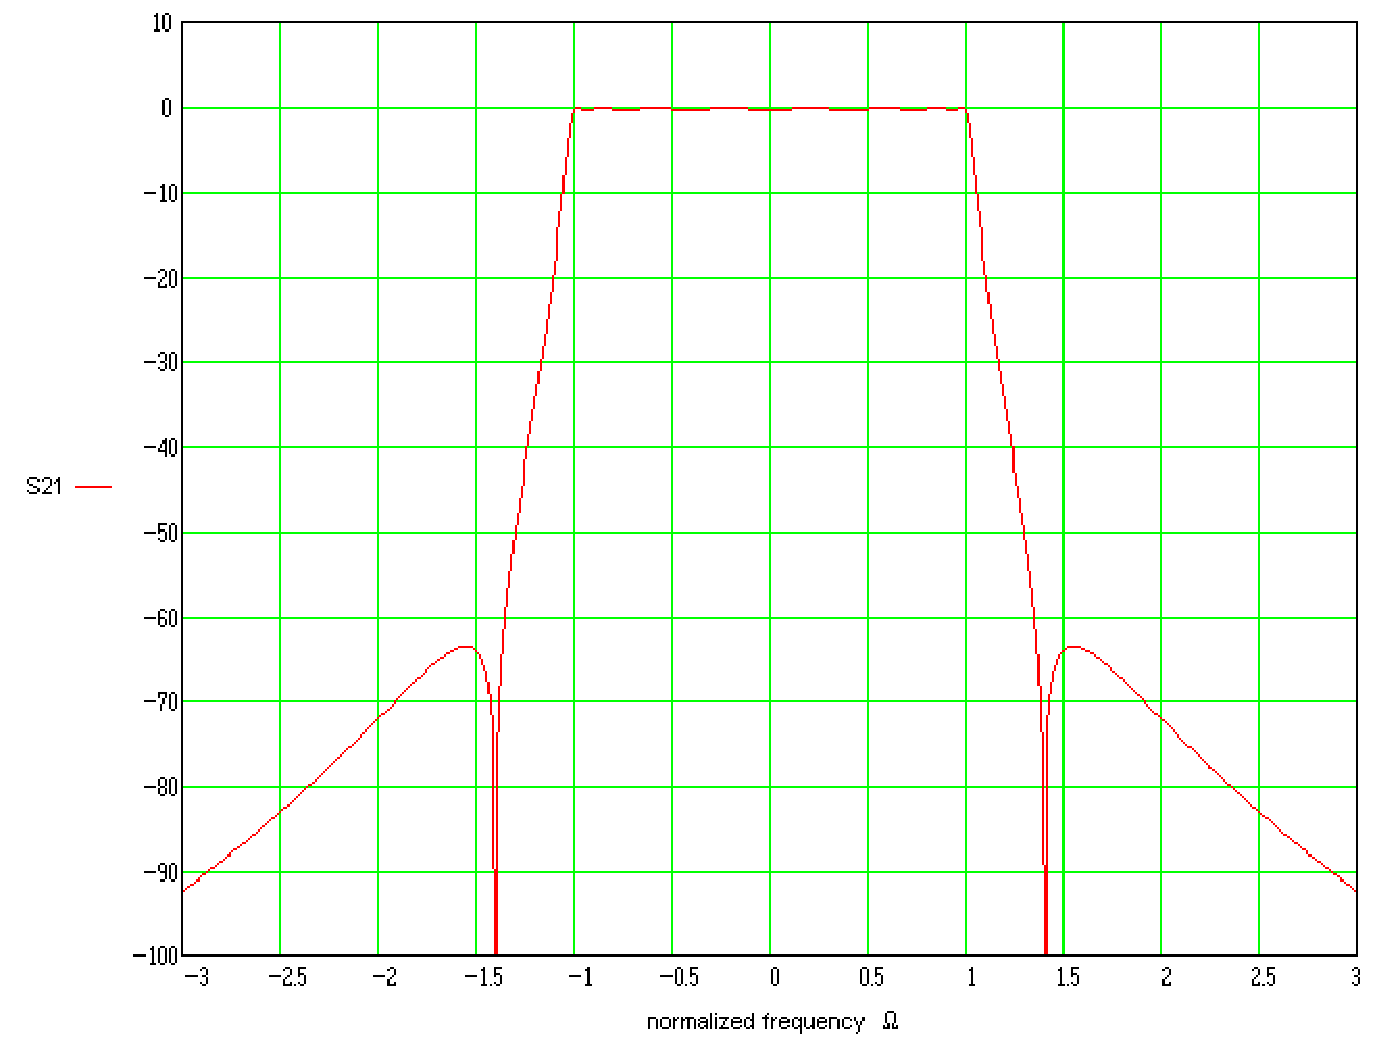
\includegraphics[scale=0.5]{fig/quazi-elliptic-8-pole-ideal.pdf}
\end{center}
\caption{8-pole quazi-elliptic filter ideal response}
\label{figure:quazi-elliptic-8-pole-ideal}

\end{figure}
The finite frequency zeros are obtained by having two separate signal paths in the filter. Figure \ref{figure:signal-paths} also shows a possible layout that includes two signal paths, the primary one through resonators 1-2-3-4-5-6-7-8, and a secondary one through 1-2-3-6-7-8. When the signals transmitted through both of these paths are $180^\circ$ out of phase at the output port, they cancel and provide the transmission zeros in the filter response.

\begin{figure}
\begin{center}
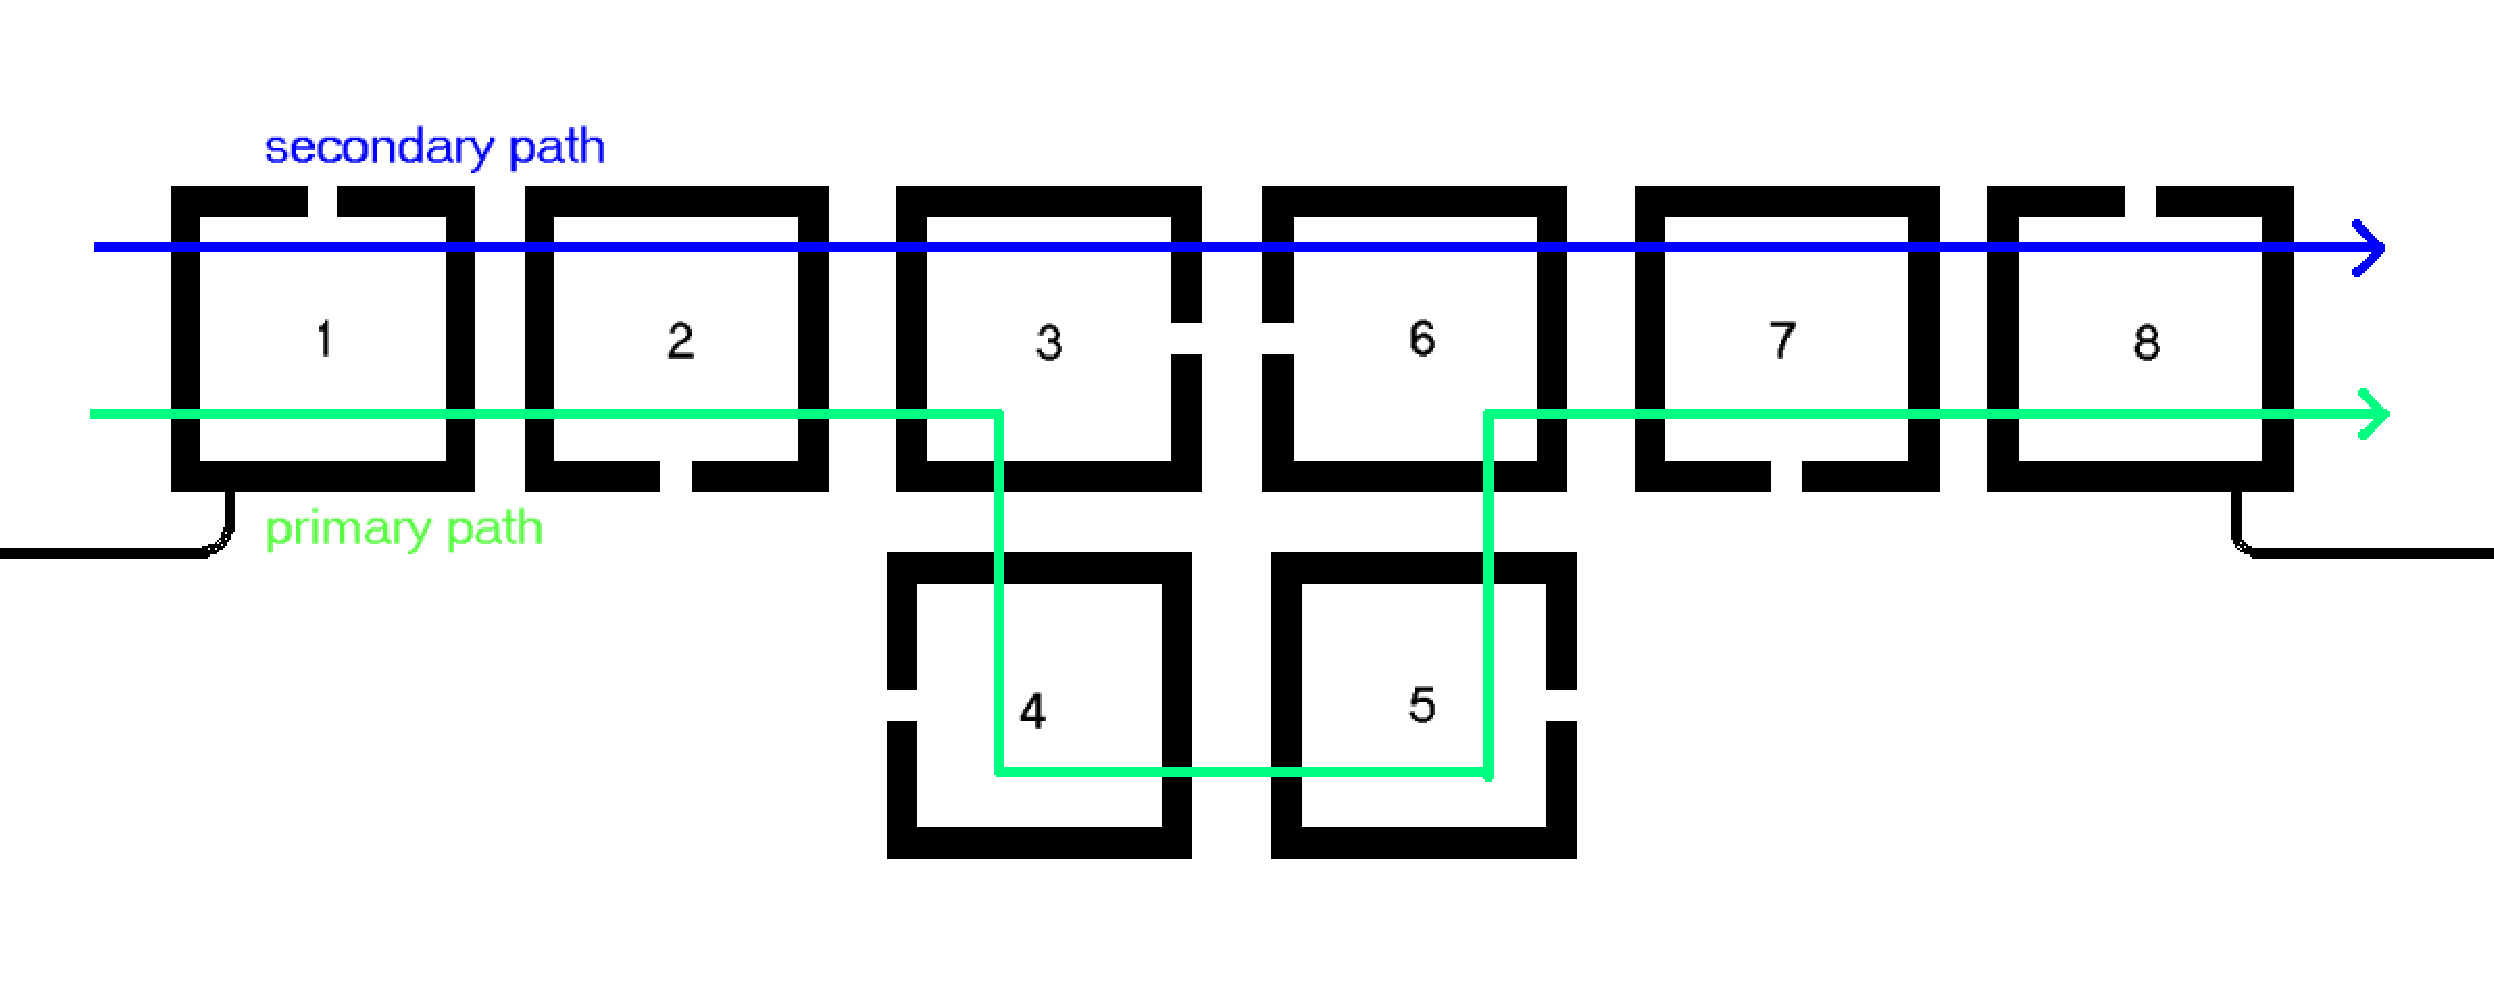
\includegraphics[scale=0.3]{fig/quazi-elliptic-8-pole-layout-path.pdf}
\end{center}
\caption{Primary and secondary signal paths}
\label{figure:signal-paths}
\end{figure}


% ------------------------------------------------------------------
\subsection{Choosing Design Parameters}
The desired filter has a passband of 2228-2292MHz with 20dB attenuation at 2300MHz. We used the filter equations of~\cite{hong:microstrip} to determine the parameters needed to meet this specification. The key parameters are the order, which is identical to the number of resonators in the circuit, and the filter parameter $\Omega_a$, which controls how close the transmission zeros are to the passband. Figure \ref{figure:filter-variation} shows the effect of changing these two parameters. Note that having zeros close to the passband provides a steeper skirt, but the two large ripples in the stop-band rise up and reduce the isolation of the filter.

We chose an 8th order filter to provide the required selectivity, while widening the design bandwidth to 68Mhz to allow some slack in the center frequency of the filter. The value of $\Omega_a$ was set to 1.4 as it provided a tradeoff between selectivity and isolation. An ideal filter with these parameters would provide 30dB attenuation at 2300MHz, which allows slack to compensate for fabrication tolerances and rounding of the response due to electrical losses.

\begin{figure}[ht]
\begin{center}
\hspace{-8em}
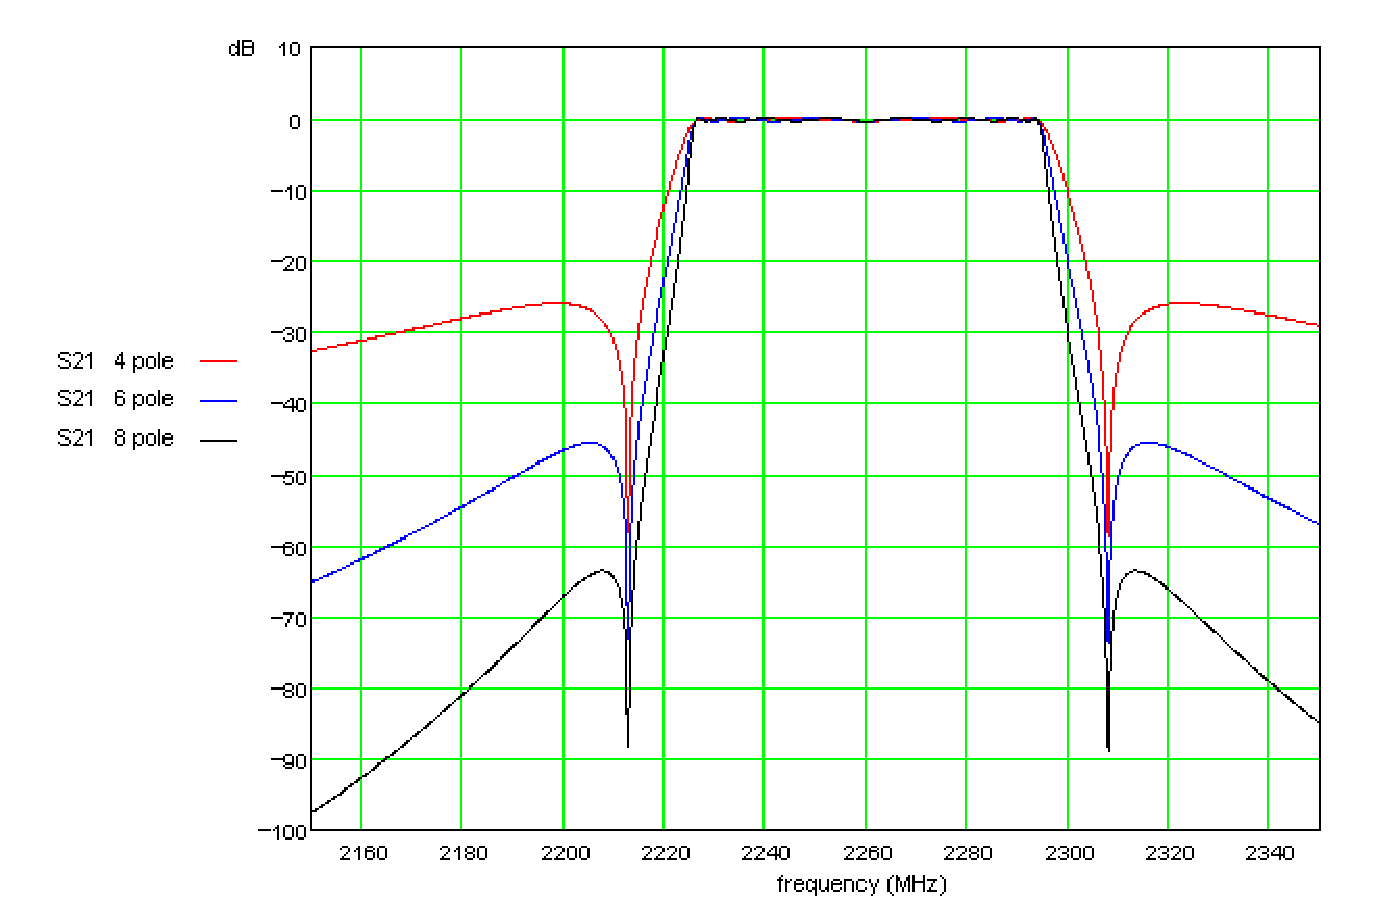
\includegraphics[scale=0.6]{fig/design-vary-order.pdf}

\hspace{-8em}
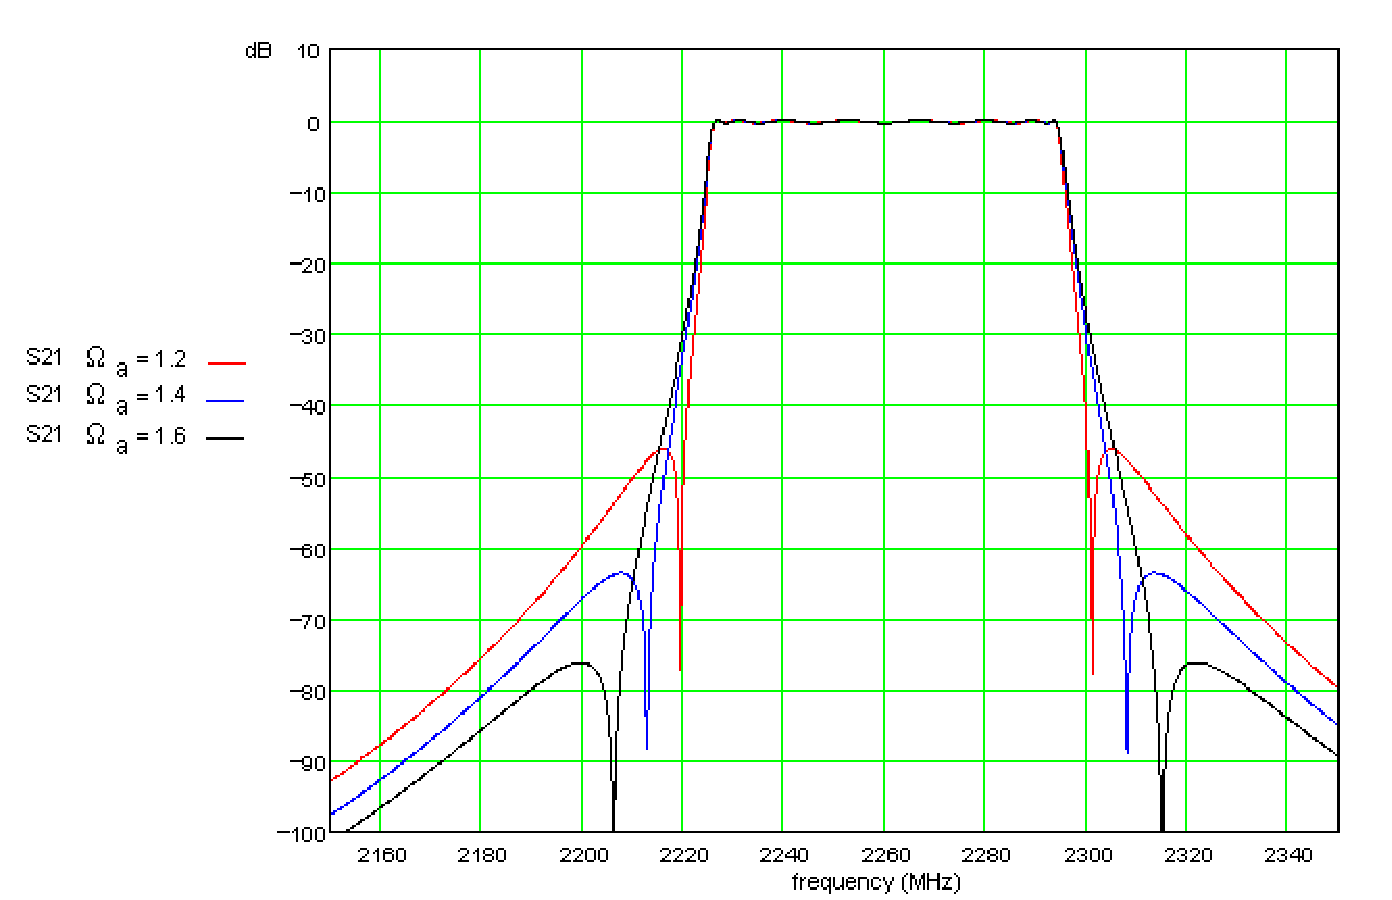
\includegraphics[scale=0.6]{fig/design-vary-omega.pdf}
\end{center}

\caption{Variations in filter response due to changing its order and $\Omega_a$}
\label{figure:filter-variation}
\end{figure}


% ------------------------------------------------------------------
\subsection{Detailed Design}
After the main parameters had been chosen, the detailed design consisted of taking one of the standard layouts and setting the length of the resonators to resonate at the desired center frequency. Next, we adjust the coupling between each pair of adjacent resonators to provide the desired quazi-elliptic response. 

In Figure~\ref{figure:signal-paths} note that there are four types of resonator couplings, where the type of coupling depends on how the resonators are arranged with respect to each other. The couplings are named electric, magnetic, mixed and hybrid, and are shown in Figure \ref{figure:design-couplings}

\begin{figure}[ht]
\begin{center}
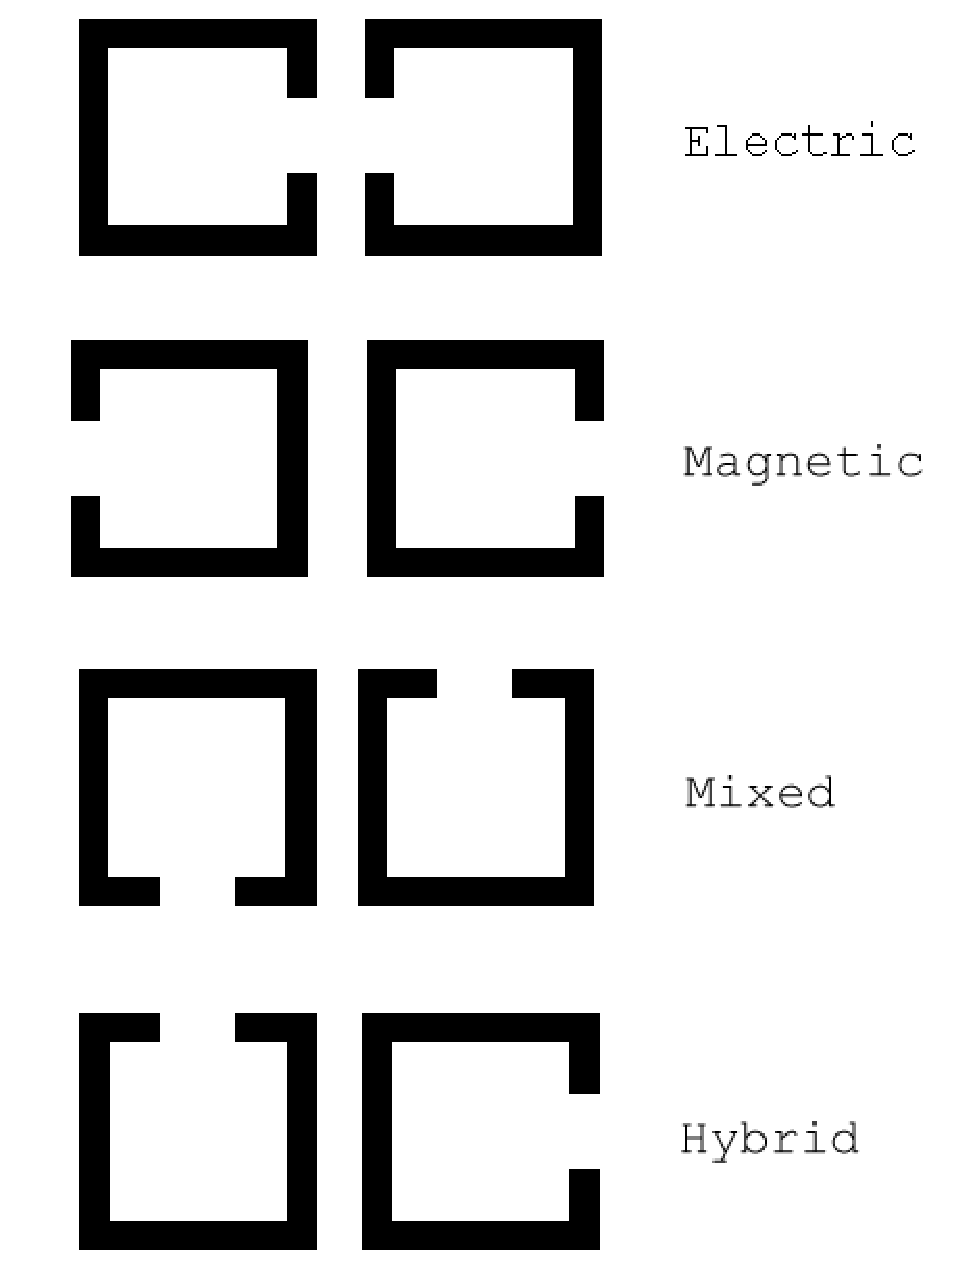
\includegraphics[scale=0.3]{fig/design-couplings.pdf}
\end{center}
\caption{Possible resonator couplings}
\label{figure:design-couplings}
\end{figure}

The coupling names ``electric'' and ``magnetic'' refer to the field that provides the coupling, and ``mixed'' and ``hybrid'' make use of both fields. An important point is that electric coupling provides a phase inversion with respect to the other types, and this is used to produce the transmission zeros in the filter response.

Once the filter layout has been chosen, the remaining design variables are the length of the resonators, and the distance between them. The resonator length sets the center frequency, and the coupling coefficents set the $\Omega_a$ parameter.


% ------------------------------------------------------------------
\subsubsection{Length of resonators}
The length of each resonator corresponds to half the wavelength at the filter's center frequency. For the copper prototype we planned to use RT Copper/Duroid 6010.5 as the substrate, which has E=10.5 and h=0.635. We used the Winline program produced by Eagleware to determine the required resonator length (about 28mm). We also used this program to calculate the width of a 50 Ohm feed line to be 0.6mm.


% ------------------------------------------------------------------
\subsubsection{Coupling coefficients}
A set of tables which state the required coupling coefficients was provided in \cite{hong:microstrip}, and \cite{hong:couplings} explains how to determine the resonator separation needed to achieve these coefficients.

Although two identical resonators have the same center frequency, when they are brought close together their fields begin to overlap. This coupled system resonates at seperate resonant frequencies, where the difference between the two frequencies increases with coupling coefficient. The coupling coefficient is determined by the proximity between the two resonators, so as they are brought closer the coefficient increases, and difference between the two resonant frequencies also increases. Figure \ref{figure:design-resonant-frequeny-splitting} shows how the filter response of two 28mm resonators varies as the separation is reduced.

\begin{figure}
\hspace{-4em}
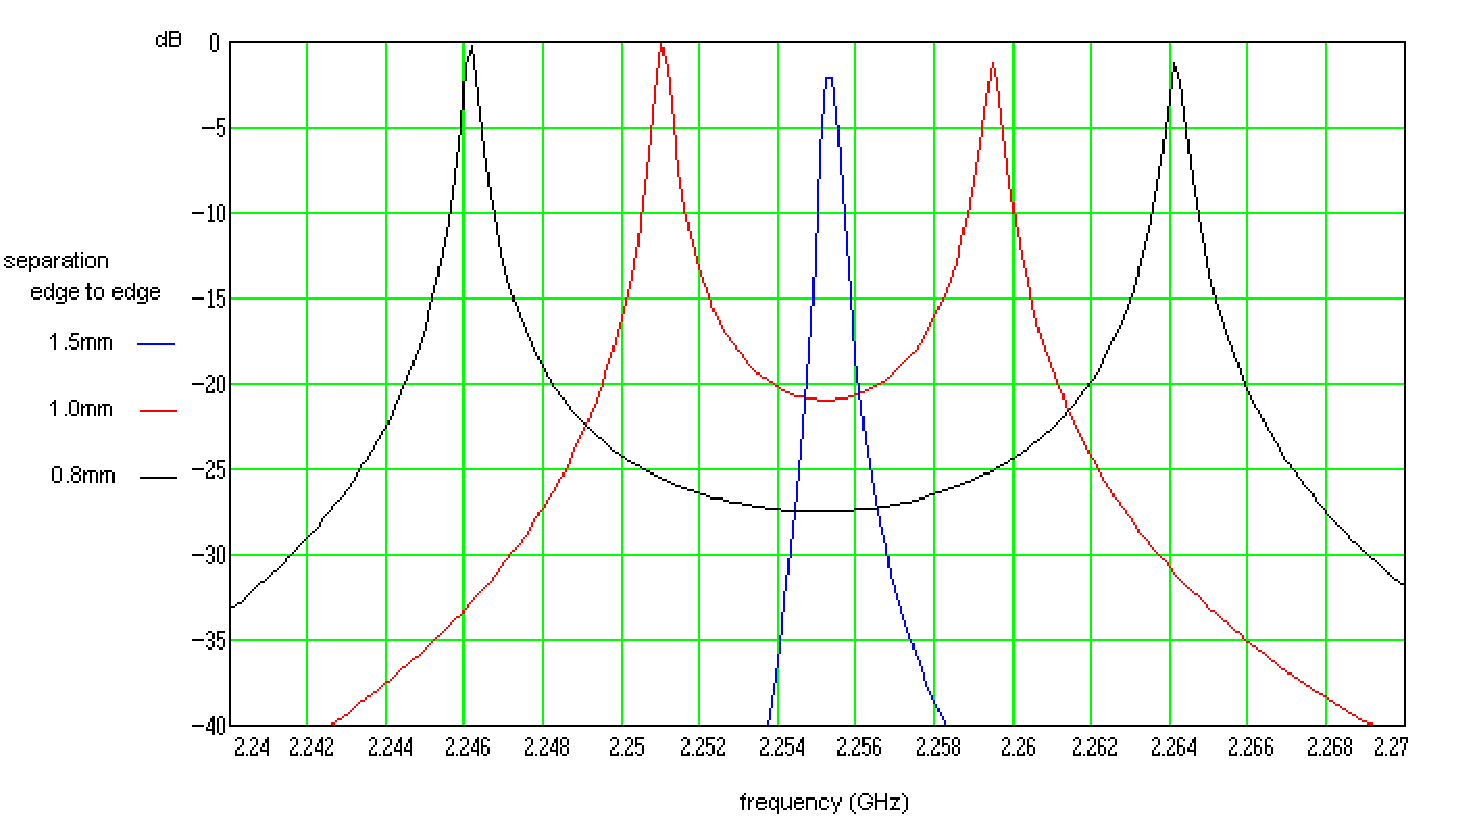
\includegraphics[scale=0.6]{fig/design-resonant-frequency-splitting.pdf}
\caption{Filter response \emph{vs} distance between coupled resonators}
\label{figure:design-resonant-frequeny-splitting}
\end{figure}

If the two resonant frequencies are $f$ and $g$, then coupling coefficient $M$ can be determined from the following equation:
$$
M = 	\frac	{f^2 - g^2}
		{f^2 + g^2}
$$

We can also control the coupling coefficient by varying the width of the resonator track, whereby reducing the width of the track increases the coupling coefficient. Note that as the resonator tracks have a finite width, there is a degree of uncertainty as to the exact length of the track seen by the resonant wave. Some trial and error is needed to determine the dimensions of the resonator. 

To determine the physical sepration required to achieve each coupling coefficient, we used the Ensemble EM simulation software by Ansoft. The process consisted of making a guess at the separation required, and then simulating a system of two coupled resonators to determine its filter response. We calculated the coupling coefficient via the above equation, and if it wasn't close enough, adjusted the separation and tried again.

Note that as the coupling between each resonator is via fringe fields, a `Full Wave' analysis package such as Ensemble must be used as it simulates the full field pattern around a planar structure. These full wave packages are different from transmission line simulators which simulate circuits via transmission line analysis, tabulated S-parameters and lumped element models for discontinuities such as corners, vias and T-sections.

We found Ensemble's simulation times to be reasonable, taking about 5 minutes to calculate 200 frequency points for two resonator circuit on Pentium II 400MHz /128MB workstation. However, as it has no automatic optimization capability, all circuit modifications had to be done by hand in the provided editor. Often the time involved in changing the circuit was more than the simulation time. Quite a few days of work could have been saved if some form of scripting language was available to set up a circuit such as in Figure~\ref{figure:design-couplings} and then take five or six frequency plots at different separations.


% ------------------------------------------------------------------
\subsubsection{Putting it together}
Once the resonator separations were determined we constructed the entire filter in Ansoft, and calculated its response. 50 Ohm lines were used to get the signal in and out of the filter, and their position along the first and last resonators determines the external Q factor of the circuit.

The first filter layout we tried, shown in Figure~\ref{figure:filter-missing-zero-layout}, had a dissapointing response. As we can see from Figure~\ref{figure:filter-missing-zero-response} the zero to the left of the pass-band is missing, and the one on the right is too high in frequency. After some investigation we decided that although arranging the resonators in this way reduces the physical size of the filter compared with the one in Figure \ref{figure:signal-paths}, it also introduces couplings between non adjacent resonators. Extra couplings such as the ones between resonators 1-3, 2-4, 3-5 and so on were not counted for in the filter design, but when simulated we determined their coefficients to be only one order of magnitude lower than the wanted couplings. Others have reported similar problems~\cite{hong:performance}. 

\begin{figure}[ht]
\begin{center}
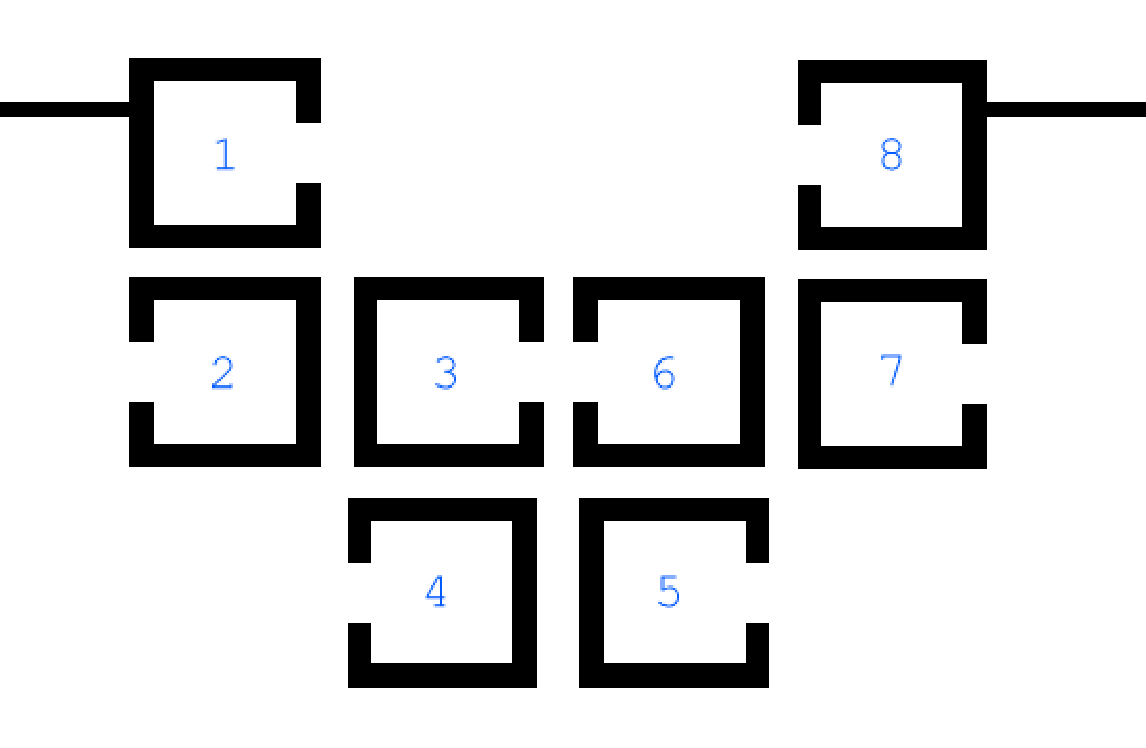
\includegraphics[scale=0.4]{fig/design-bad-8-pole-layout.pdf}
\end{center}
\caption{Filter layout with unwanted couplings}
\label{figure:filter-missing-zero-layout}
\end{figure}

\begin{figure}[ht]
\hspace{-4em}
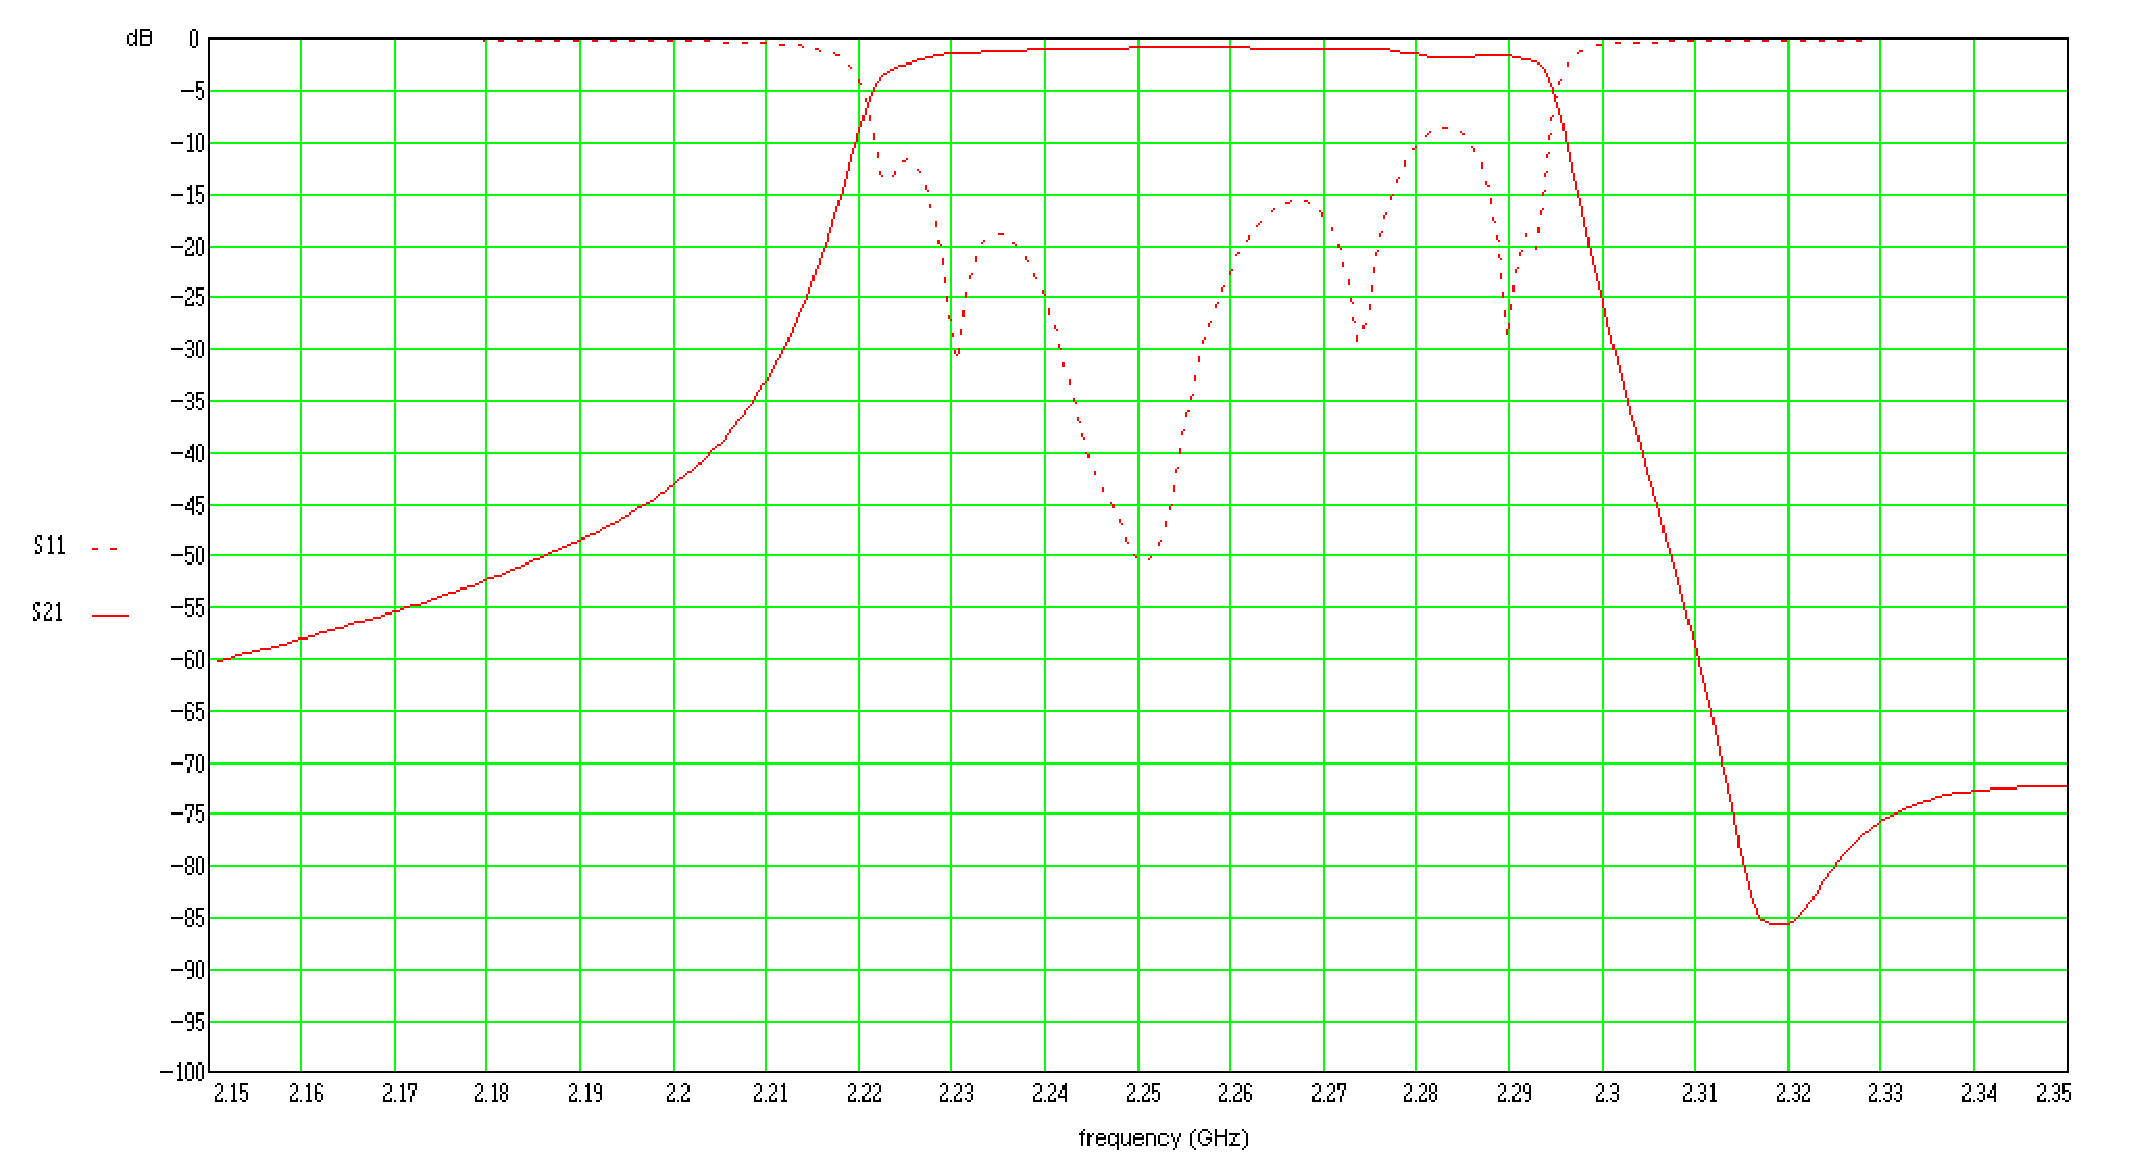
\includegraphics[scale=0.4]{fig/design-bad-8-pole-response.pdf}
\caption{Filter response with missing zero}
\label{figure:filter-missing-zero-response}
\end{figure}

To counter this problem we redesigned the filter to separate resonators 1-3 and 6-8. The final layout is shown in Figure \ref{figure:design-copper-layout} and its simulated response in Figure~\ref{figure:design-copper-response}.


\begin{figure}[ht]
\begin{center}
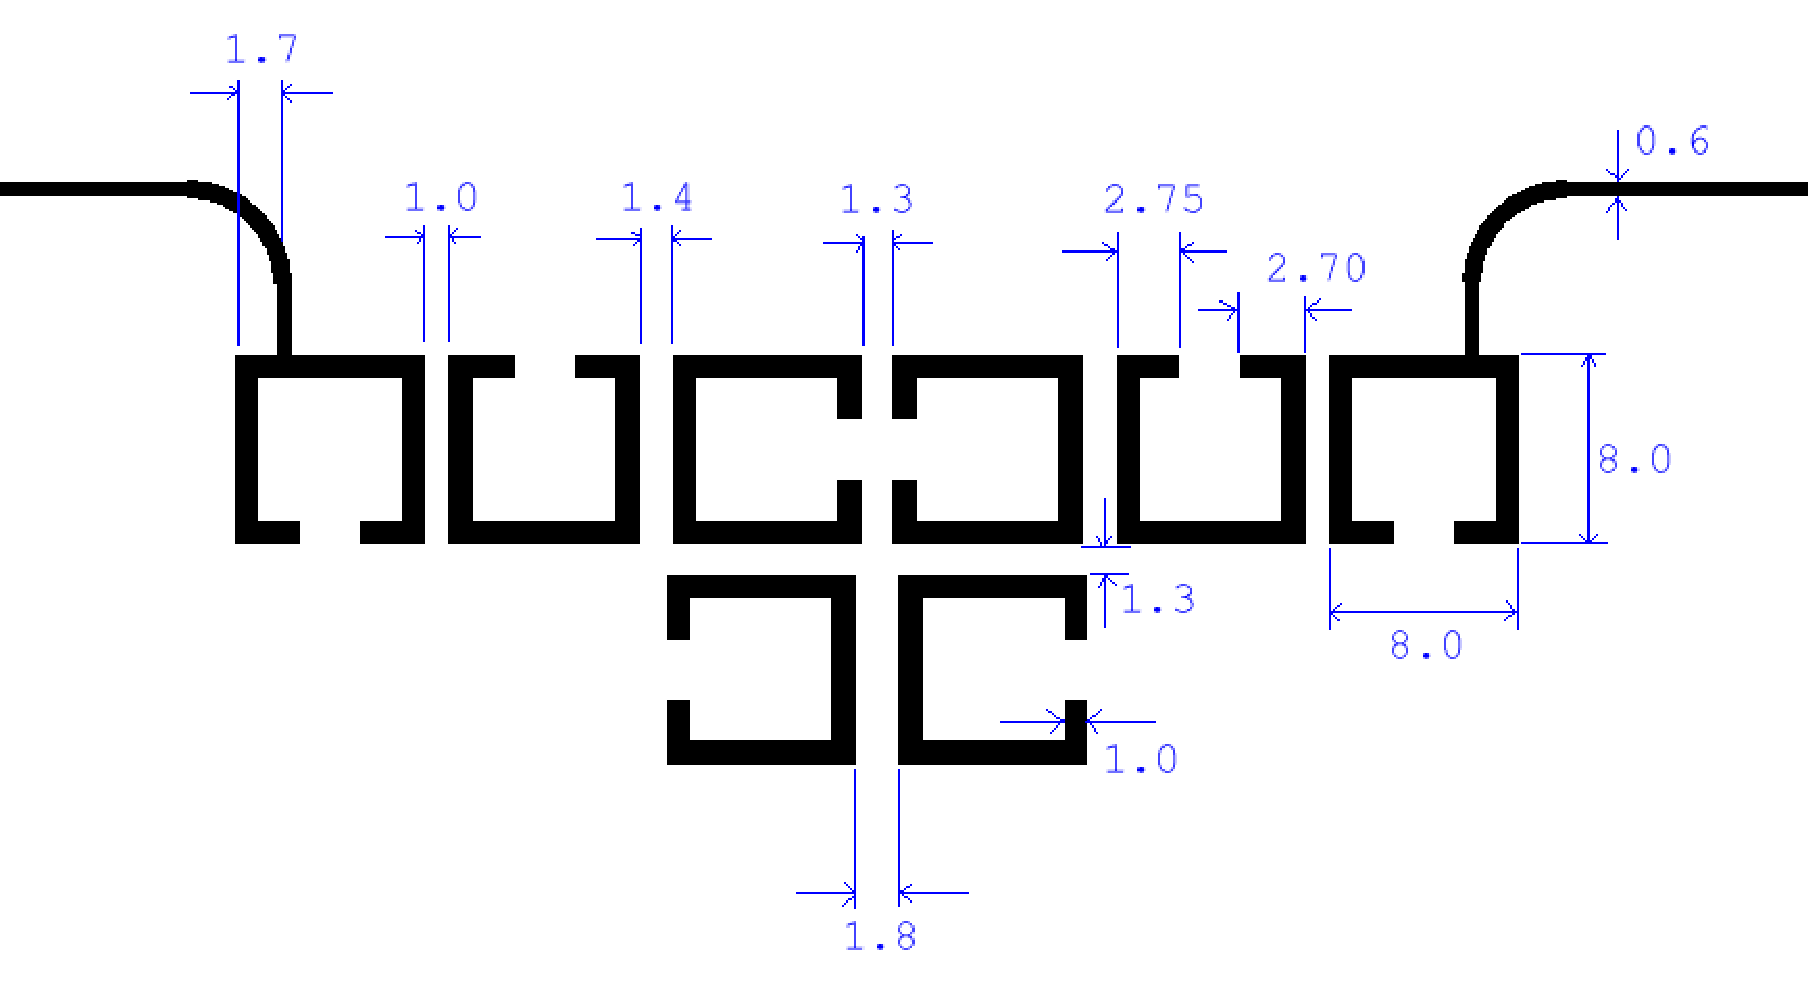
\includegraphics[scale=0.4]{fig/design-copper-layout.pdf}
\end{center}
\caption{ Final layout for copper filter (dimensions in mm)}
\label{figure:design-copper-layout}
\end{figure}

\begin{figure}[ht]
\hspace{-4em}
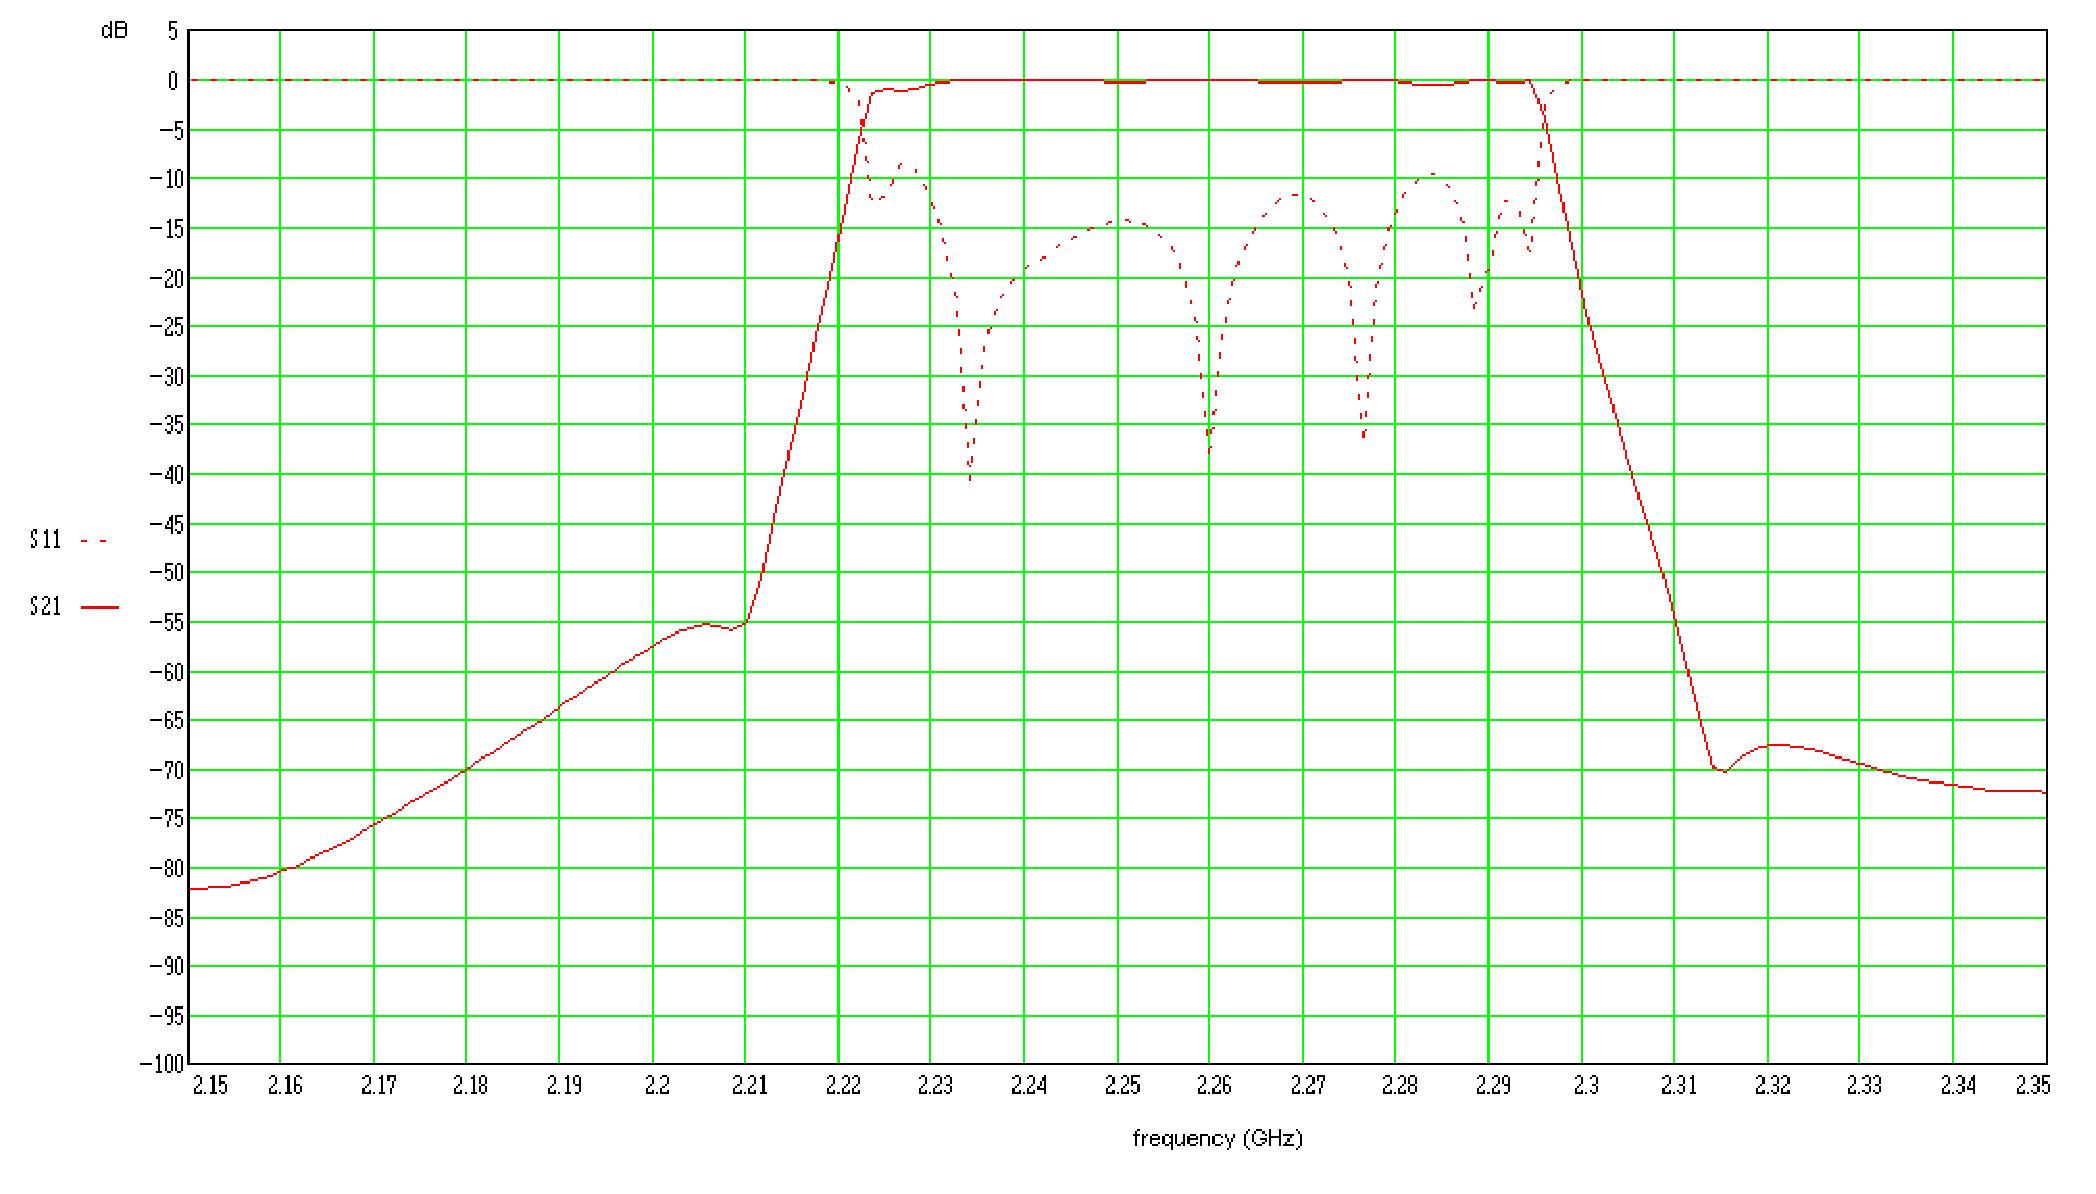
\includegraphics[scale=0.4]{fig/design-copper-simulated.pdf}
\caption{Simulated response of copper filter}
\label{figure:design-copper-response}
\end{figure}

